En graf er en samling av kanter og noder. Vi kaller mengden av alle nodene $ V $ (verticies), og mengden av alle kantene $ E $ (edges). Grafen $ G $ blir da en samling av disse to mengdene. Formelt kan vi definere en graf slik: \index{graf}

\begin{definition}
En graf $ G $  er et par $ (V, E) $, der $ V $ er en ikke-tom mengde noder og $ E $ en mengde nodepar $ \langle v_1, v_2\rangle $; $ v_1, v_2 \in V $ der $ \langle v_1, v_2\rangle $ angir at grafen inneholder en kant fra $ v_1 $ til $ v_2 $.
\end{definition}


\subsection*{Terminologi}
Vi bruker $ |E| $ for å betegne antall kanter og $ |V| $ for å betegne antall noder. \index{graf!kant}\index{graf!node}\index{node!graf}

Vi sier at en node er \textbf{nabo} med en annen node hvis de har en kant mellom seg. I figur \ref{fig:graf} er B og A naboer, men A og C er ikke naboer. \index{graf!nabo}

En \textbf{sti} eller \textbf{vei} er en sekvens av noder (og kantene mellom dem) fra en node til en annen. En sti fra A til G i figuren under kan for eksempel være A, D, C, G. (siden grafen inneholder løkker er ikke stien entydig) \index{graf!sti}\index{graf!vei}

En graf er \textbf{rettet} hvis kantene har en spesiell retning, og \textbf{urettet} hvis vi ikke bryr oss om retningen på kantene. I en rettet graf vil kanten $ \{v_1, v_2\} $ bety at det går en kant fra $ v_1 $ til $ v_2 $, men ikke nødvendigvis fra $ v_2 $ til $ v_1 $. Grafen i figur \ref{fig:tre} er urettet. Hvis en graf er rettet kaller vi ofte naboene for \textbf{etterfølgere}.  \index{graf!rettet}\index{graf!urettet}

En graf er \textbf{vektet} hvis kantene har en verdi knyttet til seg, ofte kalt \emph{kosten} til kanten. I en \textbf{uvektet} graf har ikke kantene noen spesiell verdi. Vi kan tenke på en uvektet graf som en vektet graf der alle kantene har kost = 1. \index{graf!vektet}\index{graf!uvektet}

Grafen er \textbf{syklisk} hvis den inneholder løkker, og \textbf{asyklisk} hvis den ikke inneholder løkker. I figur \ref{fig:graf} ser vi at A, B, C, D danner en løkke (det gjør også C, G, F, E). Grafen er derfor syklisk.\index{graf!syklisk}\index{graf!asyklisk}

En type grafer vi jobber mye med er \textbf{DAG}er. DAG står for \emph{Directed Asyclic Graph}, på norsk: en rettet, asyklisk graf. \index{graf!DAG}


\begin{figure}[hbt]
\centering
\caption{Eksempel på en urettet, uvektet graf}~\\
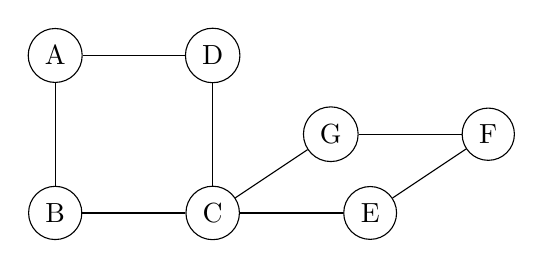
\begin{tikzpicture}
\tikzstyle{vertex} = [circle, draw=black]
\tikzstyle{edge} = [draw=black]

\node[vertex] (A) at (-1,0) {A};
\node[vertex] (B) at (-1,-2) {B};
\node[vertex] (C) at (1,-2) {C};
\node[vertex] (D) at (1,0) {D};
\node[vertex] (E) at (3,-2) {E};
\node[vertex] (F) at (4.5,-1) {F};
\node[vertex] (G) at (2.5, -1) {G};

\draw[edge] (B) -- (A);
\draw[edge] (B) -- (C);
\draw[edge] (A) -- (D);
\draw[edge] (C) -- (E);
\draw[edge] (C) -- (D);
\draw[edge] (E) -- (F);
\draw[edge] (C) -- (G);
\draw[edge] (G) -- (F);
\end{tikzpicture}
\label{fig:graf}
\end{figure}

\subsection*{Implementasjon}
Det finnes i hovedsak to måter å implementere en graf på, \textbf{Adjacency matrix} (nabomatrise) og \textbf{Adjacency list} (naboliste). Vi kan også implementere grafen som instanser av en \mono{Node}-klasse med pekere til sine naboer, men det er mindre utbredt (dette vil også være en slags implementasjon av en naboliste). Måten vi implementerer grafen på har faktisk en del å si for kompleksiteten til enkelte algoritmer.

Nabolisten til en graf er en liste over nodene og deres tilhørende naboer. Nabomatrisen er en $ n\times n $-matrise $ A $ der $ a_{i, j} $ angir vekten til kanten fra node nr $ i $ til node nr $ j $. Hvis det ikke finnes en kant er $ a_{i, j} = 0 $, og som diskutert tidligere kan en uvektet graf sees på som en vektet graf der alle vektene er 1.

For tynne grafer er nabolister klart mer plasseffektive enn nabomatriser. Nabolister gir også bedre kjøretid i enkelte algoritmer, som for eksempel \nameref{prim}, som er $ O(n^2) $ hvis grafen er representert ved en matrise, og $ O(n\log n) $ hvis grafen er representert som en liste.

\begin{figure}[htb]
	\centering
	\caption{Grafen i figur \ref{fig:graf} representert som naboliste (venstre) og nabomatrise (høyre)}
	\begin{tabular}{c | l}
		Node & Naboer \\ \hline
		A & B, D \\
		B & A, C \\
		C & B, D, G, E \\
		D & A, C \\
		E & C, F \\
		F & E, G \\
		G & C, F
	\end{tabular}\quad\quad\quad
	$ \begin{bmatrix}
	0 & 1 & 0 & 1 & 0 & 0 & 0 \\
	1 & 0 & 1 & 0 & 0 & 0 & 0 \\
	0 & 1 & 0 & 1 & 1 & 0 & 1 \\
	1 & 0 & 1 & 0 & 0 & 0 & 0 \\
	0 & 0 & 1 & 0 & 0 & 1 & 0 \\
	0 & 0 & 0 & 0 & 1 & 0 & 1 \\
	0 & 0 & 1 & 0 & 0 & 1 & 0 
	\end{bmatrix} $
\end{figure}
\noindent Merk at for en urettet graf vil nabomatrisen alltid være symmetrisk, siden at kantene går begge veier. 


